\section{Lezione 8}
\subsection{Ripasso: teoria dell'integrazione}
\begin{definition}
    \label{def:8.1}
    Sia $f\colon[a,b]\to\amsbb{R}$ una funzione \textbf{limitata definita su} $\mathbf{[a,b]}$. Una \emph{partizione} $\mathscr{P}$ di $[a,b]$ è una collezione di punti $\{x_0, \dots, x_n\}\subset [a,b]$ tale che
    \[
    a=x_0 < x_1 < \dots < x_{n-1}<x_n= b
    \]
    Data una partizione $\mathscr{P}$ di $[a,b]$ e la funzione $f$, definiamo le quantità
    \begin{equation}
        \label{eq:8.1}
        \Delta_i = x_i - x_{i-1} \qquad M_i = \sup_{x\in[x_i, x_{i-1}]} f(x) \qquad m_i = \inf_{x\in[x_i, x_{i-1}]} f(x)
    \end{equation}
    con cui definiamo la somma di Darboux superiore $U(\mathscr{P}, f)$ e inferiore $L(\mathscr{P},f)$
    \[
    \underbrace{U(\mathscr{P},f) = \sum_{i=1}^n M_i \Delta_i}_{\stepcounter{equation}\mbox{(\theequation)}} \qquad \underbrace{L(\mathscr{P},f) = \sum_{i=1}^n m_i \Delta_i}_{\stepcounter{equation}\mbox{(\theequation)}}
    \]
    \addtocounter{equation}{-2}\refstepcounter{equation}\label{eq:8.2}
    \addtocounter{equation}{0}\refstepcounter{equation}\label{eq:8.3}
\end{definition}
\begin{remark}
    Notiamo che somma superiore ed inferiore ammettono un'interessante interpretazione grafica. Nei grafici successivi riportiamo, data una generica funzione $f$ e una partizione $\mathscr{P}= \{x_0, \dots, x_6\}$ di $[a,b]$, la somma superiore $U(\mathscr{P},f)$ e inferiore $L(\mathscr{P},f)$:  
    \begin{center}
    \begin{minipage}{.45\linewidth}
        \centering
        \begin{tikzpicture}[scale=1.4, font=\footnotesize]
            \tzaxes(-1.2,-0.5)(3.3,2.7){$x$}[b]
            \tzticks{-.5/$a$, 0.6/$x_2$, 1.4/$x_4$, 2.6/$b$}[b]
            \tzticks*{-.5/$a$, 0.2/$x_1$, 0.6/$x_2$, 1.2/$x_3$, 1.4/$x_4$, 2.1/$x_5$, 2.6/$b$}
            \tzticks{0.2/$x_1$, 1.2/$x_3$, 2.1/$x_5$}[a]
            \tzfn[black]"curve"{cos(3*deg(\x))+sin(.9*deg(\x))+0.5}[-.5:2.6]{$f(x)$}[br]
            \tzpolygon*[blue,auto,dashed,text=black]
             (-0.5,0)(0.2,0)(0.2,1.5452)(-0.5,1.5452);
            \tzpolygon*[blue,auto,dashed,text=black]
             (0.2,0)(0.6,0)(0.6,1.5043)(0.2,1.5043);
            \tzpolygon*[blue,auto,dashed,text=black]
             (0.6,0)(1.2,0)(1.2,0.7869)(0.6,0.7869);
            \tzpolygon*[blue,auto,dashed,text=black]
             (1.2,0)(1.4,0)(1.4,0.9618)(1.2,0.9618);
            \tzpolygon*[blue,auto,dashed,text=black]
             (1.4,0)(2.1,0)(2.1,2.455)(1.4,2.455);
            \tzpolygon*[blue,auto,dashed,text=black]
             (2.1,0)(2.6,0)(2.6,2.4493)(2.1,2.4493);
        \end{tikzpicture}
    \end{minipage}
    \hspace{1pt}
    \begin{minipage}{.45\linewidth}
        \centering
        \begin{tikzpicture}[scale=1.4, font=\footnotesize]
            \tzaxes(-1.2,-0.5)(3.3,2.7){$x$}[b]
            \tzticks{-.5/$a$, 0.6/$x_2$, 1.4/$x_4$, 2.6/$b$}[b]
            \tzticks*{-.5/$a$, 0.2/$x_1$, 0.6/$x_2$, 1.2/$x_3$, 1.4/$x_4$, 2.1/$x_5$, 2.6/$b$}
            \tzticks{0.2/$x_1$, 1.2/$x_3$, 2.1/$x_5$}[a]
            \tzfn[black]"curve"{cos(3*deg(\x))+sin(.9*deg(\x))+0.5}[-.5:2.6]{$f(x)$}[br]
            \tzpolygon*[red,auto,dashed,text=black]
             (-0.5,0)(0.2,0)(0.2,0.1358)(-0.5,0.1358);
            \tzpolygon*[red,auto,dashed,text=black]
             (0.2,0)(0.6,0)(0.6,0.7869)(0.2,0.7869);
            \tzpolygon*[red,auto,dashed,text=black]
             (0.6,0)(1.2,0)(1.2,0.2922)(0.6,0.2922);
            \tzpolygon*[red,auto,dashed,text=black]
             (1.2,0)(1.4,0)(1.4,0.4852)(1.2,0.4852);
            \tzpolygon*[red,auto,dashed,text=black]
             (1.4,0)(2.1,0)(2.1,0.9618)(1.4,0.9618);
            \tzpolygon*[red,auto,dashed,text=black]
             (2.1,0)(2.6,0)(2.6,1.2724)(2.1,1.2724);
        \end{tikzpicture}
    \end{minipage}
\end{center}
Come si può osservare, $U(\mathscr{P}, f)$ approssima l'area sottesa dal grafico di $f$ dall'alto, mentre $L(\mathscr{P}, f)$ la approssima dal basso. Notiamo inoltre come queste due quantità dipendano sia dalla funzione $f$ considerata, sia dalla scelta della partizione $\mathscr{P}$, e che
\begin{equation}
    \label{eq:8.4}
    \left(\sup_{x\in[a,b]}f(x)\right)(b-a)\ge U(\mathscr{P}, f) \ge L(\mathscr{P},f) \ge \left(\inf_{x\in[a,b]}f(x)\right)(b-a) \ \text{per ogni} \ \mathscr{P}
\end{equation}
\end{remark}
\begin{definition}
    \label{def:8.2}
    Chiamiamo \emph{integrale inferiore} di $f$ su $[a,b]$ la quantità
    \[
    \bint_a^b f = \sup_{\mathscr{P}} L(\mathscr{P},f)
    \]
    ossia l'estremo superiore, preso su tutte le possibili partizioni $\mathscr{P}$ di $[a,b]$, dell'insieme delle somme inferiori. Analogamente, chiamiamo \emph{integrale superiore} di $f$ su $[a,b]$ la quantità
    \[
    \aint_a^b f = \inf_{\mathscr{P}} U(\mathscr{P},f)
    \]
    ossia l'estremo inferiore, preso su tutte le possibili partizioni $\mathscr{P}$ di $[a,b]$, dell'insieme delle somme superiori. Notiamo che queste due quantità sono sempre ben definite per una funzione limitata, in quanto vale la (\ref{eq:8.4}) (e ci ricordiamo il teorema \ref{th:2.1} e il corollario \ref{cor:2.1}). Diremo che $f$ è \emph{Riemann-integrabile} su $[a,b]$ ($f\in\mathscr{R}([a,b])$) se
    \[
    \bint_a^b f = \aint_a^b f
    \]
    è in tal caso il valore comune verrà denotato con
    \[
    \int_a^b f = \int_a^b f(x)\, dx 
    \]
    e verrà detto \emph{integrale di $f$ su $[a,b]$}.
\end{definition}
\begin{remark}
    Notiamo che in generale vale che
    \[
    \bint_a^b f \le \aint_a^b f
    \]
    Per mostrare la validità della disuguaglianza, procediamo come di seguito:
    \begin{enumerate}[(i)]
        \item Data una partizione $\mathscr{P}$ di $[a,b]$, un suo \emph{raffinamento} $\mathscr{Q}$ è una partizione tale che $\mathscr{P}\subseteq \mathscr{Q}$. Date due partizioni $\mathscr{P}_1$ e $\mathscr{P}_2$, il loro raffinamento comune sarà dato da $\mathscr{P}_1 \cup \mathscr{P}_2$.
        \item Se $\mathscr{Q}$ è un raffinamento di $\mathscr{P}$, allora vale che
        \[
        L(\mathscr{P}, f) \le L(\mathscr{Q},f) \qquad U(\mathscr{Q},f)\le U(\mathscr{P},f)
        \]
        Per mostrare che valgono queste due disuguaglianze, consideriamo il caso base in cui $\mathscr{Q} = \mathscr{P} \cup \{\overline{x}\}$, $x_{i-1} < \overline{x}<x_i$ per qualche $i$. Definiamo
        \[
        \overline{m}_1 = \inf_{x\in[x_{i-1}, \overline{x}]}f(x) \qquad \overline{m}_2 = \inf_{x\in[\overline{x}, x_i]}f(x)
        \]
        e notiamo che
        \[
        \overline{m}_1 \ge m_i \qquad \overline{m}_2 \ge m_i
        \]
        A questo punto vale che
        \[
        \begin{split}
            L(\mathscr{Q}, f)-L(\mathscr{P},f) &= \sum_{k=1}^{i-1}m_k \Delta_k + \overline{m}_1 (\overline{x}-x_{i-1}) + \overline{m}_2 (x_i - \overline{x}) + \sum_{k=i+1}^n m_k \Delta_k - \\
            & -\sum_{k=1}^n m_k \Delta_k = \overline{m}_1 (\overline{x}-x_{i-1}) + \overline{m}_2 (x_i - \overline{x})-m_i(x_{i}-x_{i-1})\ge \\
            & \ge m_i(\overline{x}-x_{i-1}) + m_i (x_i -\overline{x})-m_i(x_i-x_{i-1}) = 0
        \end{split}
        \]
        Il risultato si dimostra analogamente per $U(\mathscr{Q}, f) \le U(\mathscr{P},f)$.
        \item Per il punto precedente vale che, date due generiche partizioni $\mathscr{P}_1$ e $\mathscr{P_2}$ e indicando con $\mathscr{Q}$ il loro raffinamento comune,
        \[
        L(\mathscr{P}_1, f)\le L(\mathscr{Q}, f) \le U(\mathscr{Q}, f)\le U(\mathscr{P_2}, f)
        \]
        ossia
       \begin{equation}
           \label{eq:8.5}
           L(\mathscr{P}_1, f)\le U(\mathscr{P}_2, f) \ \text{per ogni} \ \mathscr{P}_1, \mathscr{P}_2
       \end{equation}
       Fissiamo a questo punto $\mathscr{P}_1$; vale che
       \[
       L(\mathscr{P}_1, f)\le U(\mathscr{P}_2, f) \ \forall \mathscr{P}_2 \implies L(\mathscr{P}_1, f)\le \aint_a^b f
       \]
       Poiché la partizione $\mathscr{P}_1$ che avevamo fissato era generica, allo stesso modo vale che
       \[
       L(\mathscr{P}_1, f)\le \aint_a^b f \ \forall \mathscr{P}_1 \implies \bint_a^b f \le \aint_a^b f
       \]
    \end{enumerate}
\end{remark}
\begin{theorem}[Criterio di Riemann]
    \label{th:8.1}
    Una funzione $f\colon [a,b]\to \amsbb{R}$ limitata su $[a,b]$ è Riemann-integrabile se e solo se per ogni $\varepsilon>0$ esiste una partizione $\mathscr{P}_\varepsilon$ di $[a,b]$ tale che
    \[
    U(\mathscr{P}_\varepsilon, f) - L(\mathscr{P}_\varepsilon, f)< \varepsilon
    \]
\end{theorem}
\begin{proof}
    Mostriamo le due implicazioni.
    \begin{enumerate}[(i)]
        \item Supponiamo che $f\in\mathscr{R}([a,b])$. Notiamo che per ogni partizione $\mathscr{P}$ di $[a,b]$ vale che
        \[
        L(\mathscr{P},f) \le \bint_a^b f \le \aint_a^b f \le U(\mathscr{P}, f)
        \]
        Per definizione (cfr. definizione \ref{def:2.2}) di estremo superiore, per ogni $\varepsilon>0$ esiste una partizione $\mathscr{P}_1$ tale che
        \[
        L(\mathscr{P}_1, f) > \bint_a^b f -\frac{\varepsilon}{2} \iff L(\mathscr{P}_1, f) + \frac{\varepsilon}{2}> \bint_a^b f
        \]
        e allo stesso modo per definizione di estremo inferiore per ogni $\varepsilon>0$ esiste una partizione $\mathscr{P}_2$ tale che
        \[
        U(\mathscr{P}_2, f) < \aint_a^b f +\frac{\varepsilon}{2} \iff U(\mathscr{P}_2, f) - \frac{\varepsilon}{2}<\aint_a^b f
        \]
        Definiamo $\mathscr{P}_\varepsilon = \mathscr{P_1}\cup \mathscr{P}_2$; vale che
        \[
        U(\mathscr{P}_\varepsilon, f) \le U(\mathscr{P}_2, f) < \underbrace{\bint_a^bf +\frac{\varepsilon}{2} = \aint_a^b f -\frac{\varepsilon}{2}+\varepsilon}_{\text{Definizione \ref{def:8.2}}} < L(\mathscr{P}_1, f)+\varepsilon \le L(\mathscr{P}_\varepsilon, f) + \varepsilon
        \]
        ossia abbiamo trovato, per ogni $\varepsilon>0$, una partizione $\mathscr{P}_\varepsilon$ tale che
        \[
        U(\mathscr{P}_\varepsilon, f) < L(\mathscr{P}_\varepsilon, f) + \varepsilon \iff U(\mathscr{P}_\varepsilon, f) - L(\mathscr{P}_\varepsilon, f) <  \varepsilon
        \]
        \item Supponiamo che per ogni $\varepsilon>0$ esista una partizione $\mathscr{P}_\varepsilon$ tale che
        \[
        U(\mathscr{P}_\varepsilon, f) - L(\mathscr{P}_\varepsilon, f)< \varepsilon
        \]
        Sappiamo che $U(\mathscr{P}_\varepsilon, f)\ge \aint_a^b f$ e che $L(\mathscr{P}_\varepsilon, f)\le \bint_a^b f$; quindi
        \[
        \varepsilon>U(\mathscr{P}_\varepsilon, f) - L(\mathscr{P}_\varepsilon, f) \ge \aint_a^b f - L(\mathscr{P}_\varepsilon, f) \ge \underbrace{\aint_a^b f - \bint_a^b f\ge 0}_{\text{Osservazione precedente}}
        \]
        ossia per ogni $\varepsilon>0$,
        \[
        0\le \aint_a^b f - \bint_a^b <\varepsilon
        \]
        Ma questo significa che
        \[
        0\le \aint_a^b f - \bint_a^b \le 0 \iff \aint_a^b f = \bint_a^b
        \]
        e quindi $f$ soddisfa la definizione \ref{def:8.2}.\qedhere
    \end{enumerate}
\end{proof}
\begin{corollary}
    \label{cor:8.1}
    Data una funzione $f\colon[a,b]\to \amsbb{R}$, $f\in\mathscr{R}([a,b])$ se soddisfa una delle seguenti proprietà:
    \begin{enumerate}[(i)]
        \item $f$ è continua su $[a,b]$;
        \item $f$ è monotona su $[a,b]$;
        \item $f$ è limitata su $[a,b]$ ed ha al più un numero finito di discontinuità.
    \end{enumerate}
    Inoltre, se $f,g\in\mathscr{R}([a,b])$ vale che
    \begin{enumerate}[(i)]
        \item $f+g\in\mathscr{R}([a,b])$ e 
        \[
        \int_a^b f+g = \int_a^b f + \int_a^b g
        \]
        \item $\lambda f\in\mathscr{R}([a,b])$ per ogni $\lambda\in\amsbb{R}$, e
        \[
        \int_a^b \lambda f = \lambda \int_a^b f
        \]
        \item $fg\in\mathscr{R}([a,b])$;
        \item $\abs{f}\in\mathscr{R}([a,b])$ e
        \[
        \abs{\int_a^b f} \le \int_a^b \abs{f}
        \]
        \item Se $a<c<b$, allora $f\in\mathscr{R}([a,c])$ e $f\in\mathscr{R}([c,b])$ e
        \[
        \int_a^b f = \int_a^c f + \int_c^b f
        \]
    \end{enumerate}
\end{corollary}
\begin{corollary}
    \label{cor:8.2}
    Sia $f\colon [a,b]\to \amsbb{R}$ una funzione Riemann-integrabile su $[a,b]$, e sia $\widehat{f}\colon[a,b]\to \amsbb{R}$ definita da
    \[
    \widehat{f}(x) = \begin{dcases}
        f(x)\, & x\ne \overline{x}\\
        k\ne f(\overline{x})\, & x=\overline{x}
    \end{dcases}
    \]
    per qualche $\overline{x}\in[a,b]$. Allora $\widehat{f}\in \mathscr{R}([a,b])$ e 
    \[
    \int_a^b f = \int_a^b \widehat{f}
    \]
\end{corollary}
\begin{proof}
    Consideriamo come primo caso $f\equiv 0$ su $[a,b]$, e quindi
    \[
    \widehat{f}(x) = \begin{dcases}
        0\, & x\ne \overline{x}\\
        M\, & x=\overline{x}
    \end{dcases}
    \]
    con $M>0$ per semplicità. Data la forma di $f$, sappiamo che se consideriamo la partizione $\mathscr{P}=\{x_0 = a, x_1 = b\}$ vale che
    \[
    U(\mathscr{P}, f) -L(\mathscr{P}, f) <\varepsilon
    \]
    per ogni possibile scelta di $\varepsilon>0$. \\
    Consideriamo ora un $\varepsilon>0$ fissato; vogliamo utilizzare il criterio di Riemann \ref{th:8.1} per dimostrare che $\widehat{f}\in\mathscr{R}([a,b])$. A questo scopo, definiamo la partizione
    \[
    \mathscr{P}_\varepsilon = \left\{x_0, \overline{x}-\frac{\varepsilon}{4M}, \overline{x}+\frac{\varepsilon}{4M}, x_1\right\}
    \]
    e calcoliamo $U(\mathscr{P}_\varepsilon, \widehat{f})$ e $L(\mathscr{P}_\varepsilon, \widehat{f})$: vale che
    \[
    U(\mathscr{P}_\varepsilon, \widehat{f}) = \sup_{x\in \left[\overline{x}-\frac{\varepsilon}{4M}, \overline{x}+\frac{\varepsilon}{4M}\right]} \widehat{f}(x) = M \frac{\varepsilon}{2M} = \frac{\varepsilon}{2}<\varepsilon
    \]
    e che
    \[
    L(\mathscr{P}_\varepsilon, \widehat{f}) = 0 
    \]
    Di conseguenza 
    \[
    U(\mathscr{P}_\varepsilon, \widehat{f}) - L(\mathscr{P}_\varepsilon, \widehat{f})<\varepsilon 
    \]
    e quindi $\widehat{f}\in\mathscr{R}([a,b])$. Per dimostrare che
    \[
    \int_a^b \widehat{f} = \int_a^b f = 0
    \]
    notiamo che, seguendo il ragionamento visto prima, per ogni $\varepsilon>0$ riusciamo a trovare una partizione $\mathscr{P}_\varepsilon$ tale che 
    \[
    U(\mathscr{P}_\varepsilon, \widehat{f})<\varepsilon
    \]
    Di conseguenza, poiché
    \[
    0= L(\mathscr{P}_\varepsilon, \widehat{f}) \le \bint_a^b \widehat{f} = \aint_a^b \widehat{f} \le U(\mathscr{P}_\varepsilon, \widehat{f})<\varepsilon
    \]
    possiamo dire che
    \[
    0\le \int_a^b \widehat{f} < \varepsilon \ \text{per ogni} \ \varepsilon>0
    \]
    ossia $\int_a^b \widehat{f} = 0$. Analogo risultato vale se $\widehat{f}(\overline{x})<0$.\\
    Per quanto riguarda invece il nostro asserto originario, notiamo che data una generica funzione $f\in\mathscr{R}([a,b])$ possiamo scrivere
    \[
    \widehat{f} = f + \underbrace{\widehat{f}-f}_{g}
    \]
    $g(x)$ è una funzione con le proprietà sopra descritte; pertanto $g\in\mathscr{R}([a,b])$ e $\int_a^b g = 0$. Usando il corollario \ref{cor:8.1} abbiamo quindi che $f+g = \widehat{f}\in\mathscr{R}([a,b])$ e che
    \[
    \int_a^b f = \int_a^b f + \int_a^b g = \int_a^b(f+g) = \int_a^b \widehat{f}
    \]
\end{proof}
\begin{remark}
    Il corollario \ref{cor:8.2} ci dice che l'integrazione secondo Riemann non dipende dal valore di una funzione in un numero $n$ arbitrario (ma finito!) di punti.
\end{remark}
\begin{theorem}
    \label{th:8.2}
    Sia $f\colon\mathscr{R}([a,b])$, e $x\in[a,b]$; se definiamo
    \begin{equation}
        \label{eq:8.6}
        F(x) = \int_a^xf(t)\, dt
    \end{equation}
    $F$ è continua in $[a,b]$; inoltre, se $f$ è continua in $x_0\in[a,b]$ allora $F$ è differenziabile in $x_0$ e $F'(x_0) = f(x_0)$.
\end{theorem}
\begin{proof}
    Notiamo che $F$ è ben definita per il corollario \ref{cor:8.1}, punto (v).\\
    Fissiamo $x\in[a,b]$; vogliamo mostrare che per ogni $\varepsilon>0$ esiste $\delta_\varepsilon>0$ tale che
    \[
    \abs{F(x)-F(y)}<\varepsilon \ \text{se} \ \abs{x-y}<\delta_\varepsilon
    \]
    Possiamo supporre $y<x$; allora per il corollario \ref{cor:8.1} vale che
    \[
    \abs{F(x)-F(y)} = \abs{\int_a^x f - \int_a^y f} \overset{\text{(v)}}{=} \abs{\int_x^y f} \overset{\text{(iv)}}{\le }\int_x^y \abs{f}
    \]
    Ricordiamo che $f$ è una funzione limitata, ossia
    \[
    \abs{f(x)} \le M \ \text{per ogni} \ x\in[a,b]
    \]
    Quindi
    \[
    \abs{F(x)-F(y)} {\le }\int_x^y \abs{f} \le M (x-y)
    \]
    Quindi se prendiamo $\delta_\varepsilon = \frac{\varepsilon}{2M}$ abbiamo che
    \[
    \abs{F(x)-F(y)}<\varepsilon \ \text{se} \ \abs{x-y}<\delta_\varepsilon
    \]
    E di conseguenza $F$ è continua in $x$; poiché $x\in[a,b]$ è generico, $F$ è continua in $[a,b]$.\\
    Supponiamo ora che $f$ sia continua in $x_0\in[a,b]$; allora per ogni $\varepsilon>0$ esiste $\delta_\varepsilon>0$ tale che
    \begin{equation}
        \label{eq:8.7}
        \abs{f(x_0)-f(t)}<\varepsilon \ \text{se} \ \abs{x_0-t}<\delta_\varepsilon
    \end{equation}
    Vogliamo mostrare che $F$ è differenziabile in $x_0$, ossia (cfr. definizione \ref{def:6.1}) che 
    \[
    \lim_{t\to x_0} \frac{F(t)-F(x_0)}{t-x_0} = f(x_0)
    \]
    Fissiamo quindi $\varepsilon>0$, e consideriamo
    \[
    \begin{split}
        & \abs{\frac{F(t)-F(x_0)}{t-x_0}-f(x_0)} = \abs{\frac{1}{t-x_0}\int_{x_0}^tf -\frac{t-x_0}{t-x_0}f(x_0)} = \abs{\frac{1}{t-x_0} \int_{x_0}^t f - \frac{f(x_0)}{t-x_0}\int_{x_0}^t} = \\
        & = \abs{\frac{1}{t-x_0}\int_{x_0}^t (f-f(x_0))}\le \frac{1}{\abs{t-x_0}}\int_{x_0}^t\abs{f(u)-f(x_0)}\, du \overset{(\ref{eq:8.6})}{<}\frac{1}{\abs{t-x_0}}\int_{x_0}^t \varepsilon = \varepsilon
    \end{split}
    \]
    se $\abs{t-x_0}<\delta_\varepsilon$, in quanto in questo caso $\abs{u-x_0}<\delta_\varepsilon$ per ogni $u\in[x_0,t]$. Quindi dato $\varepsilon>0$ abbiamo trovato $\delta_\varepsilon$ tale che
    \[
    \abs{\frac{F(t)-F(x_0)}{t-x_0}-f(x_0)}<\varepsilon \ \text{se} \ \abs{t-x_0}<\delta_\varepsilon
    \]
    ossia vale, come richiesto, 
    \[
    \lim_{t\to x_0} \frac{F(t)-F(x_0)}{t-x_0} = f(x_0)
    \]
\end{proof}
\begin{remark}
    La funzione $F$ definita nell'equazione (\ref{eq:8.6}) è detta \emph{funzione integrale} di $f$.
\end{remark}
\begin{theorem}[Teorema fondamentale del calcolo]
    \label{th:8.3}
    Sia $f\in\mathscr{R}([a,b])$; se esiste una funzione $F\colon[a,b]\to \amsbb{R}$ tale che $F'=f$, allora
    \[
    \int_a^b f(x)\, dx = F(b)-F(a)
    \]
\end{theorem}
\begin{proof}
    Per il criterio di Riemann \ref{th:8.1} sappiamo che per ogni $\varepsilon>0$ esiste una partizione $\mathscr{P}_\varepsilon$ tale che 
    \[
    U(\mathscr{P}_\varepsilon, f) - L(\mathscr{P}_\varepsilon, f)<\varepsilon
    \]
    Tale partizione è data da $\mathscr{P}_\varepsilon = \{x_0, x_1, \dots, x_i, \dots, x_n\}$. Consideriamo ora $F\Big|_{[x_{i-1}, x_i]}$; poiché $F$ è differenziabile su (un aperto contenente) $[a,b]$, lo è in $(x_{i-1}, x_i)$, ed è inoltre continua in $[x_{i-1}, x_i]$. Pertanto possiamo applicare il teorema di Lagrange \ref{th:7.2}: esiste $t_i\in(x_{i-1}, x_i)$ tale che
    \[
    F(x_i) -F(x_{i-1}) = f(t_i) (x_i - x_{i-1})
    \]
    Notiamo quindi che
    \[
    \sum_{i=1}^n F(x_i) -F(x_{i-1}) = F(b)-F(a)
    \]
    Consideriamo
    \[
    \sum_{i=1}^nf(t_i) \Delta_i
    \]
    Notiamo che $m_i \le f(t_i) \le M_i $, e di conseguenza
    \[
    L(\mathscr{P}_\varepsilon, f) \le F(b)-F(a) \le U(\mathscr{P}_\varepsilon, f)
    \]
    Ricordando che 
    \[
    L(\mathscr{P}, f) \le \int_a^b f \le U(\mathscr{P}, f) \ \text{per ogni partizione}\ \mathscr{P}
    \]
    possiamo scrivere
    \[
    \left(F(b)-F(a)\right)-\int_a^bf \le \left(F(b)-F(a)\right)-L(\mathscr{P}_\varepsilon, f) \le U(\mathscr{P}_\varepsilon, f)-L(\mathscr{P}_\varepsilon, f) < \varepsilon
    \]
    e
    \[
    \int_a^b f -\left(F(b)-F(a)\right)\le U(\mathscr{P}_\varepsilon, f) - \left(F(b)-F(a)\right) \le U(\mathscr{P}_\varepsilon, f) - L(\mathscr{P}_\varepsilon, f) <\varepsilon
    \]
    ossia
    \[
    \abs{\left(F(b)-F(a)\right)-\int_a^bf}<\varepsilon
    \]
    per ogni $\varepsilon>0$; ciò implica che
    \[
    \abs{\left(F(b)-F(a)\right)-\int_a^bf} = 0 \iff F(b)-F(a)=\int_a^bf
    \]
\end{proof}
\begin{remark}
    Una funzione $F$ avente le proprietà descritte dall'enunciato del teorema \ref{th:8.3} è detta \emph{primitiva} di $f$.\\ 
    Il teorema fondamentale del calcolo \ref{th:8.3} è la ragione per cui si ricercano le primitive delle funzioni per calcolare gli integrali.
\end{remark}
\subsection{Esercizi: ricerca delle primitive}
